
%% Package and Class "uiucthesis2014" for use with LaTeX2e.
\documentclass{article}

\usepackage[acronym,toc]{glossaries}
%\newacronym{<++>}{<++>}{<++>}
\newacronym[longplural={metric tons of heavy metal}]{MTHM}{MTHM}{metric ton of heavy metal}
\newacronym{ABM}{ABM}{agent-based modeling}
\newacronym{ACDIS}{ACDIS}{Program in Arms Control \& Domestic and International Security}
\newacronym{ADS}{ADS}{Accelerator-Driven Systems}
\newacronym{AHTR}{AHTR}{Advanced High Temperature Reactor}
\newacronym{ANDRA}{ANDRA}{Agence Nationale pour la gestion des D\'echets RAdioactifs, the French National Agency for Radioactive Waste Management}
\newacronym{ANL}{ANL}{Argonne National Laboratory}
\newacronym{ANS}{ANS}{American Nuclear Society}
\newacronym{API}{API}{application programming interface}
\newacronym{ARE}{ARE}{Aircraft Reactor Experiment}
\newacronym{ARFC}{ARFC}{Advanced Reactors and Fuel Cycles}
\newacronym{ASME}{ASME}{American Society of Mechanical Engineers}
\newacronym{ASTRID}{ASTRID}{Advanced Sodium Technological Reactor for Industrial Demonstration}
\newacronym{ATWS}{ATWS}{Anticipated Transient Without Scram}
\newacronym{BDBE}{BDBE}{Beyond Design Basis Event}
\newacronym{BIDS}{BIDS}{Berkeley Institute for Data Science}
\newacronym{BWR}{BWR}{Boiling Water Reactor}
\newacronym{CAFCA}{CAFCA}{ Code for Advanced Fuel Cycles Assessment }
\newacronym{CANDU}{CANDU}{Canada Deuterium Uranium}
\newacronym{CDTN}{CDTN}{Centro de Desenvolvimento da Tecnologia Nuclear}
\newacronym{CEA}{CEA}{Commissariat \`a l'\'Energie Atomique et aux \'Energies Alternatives}
\newacronym{CI}{CI}{continuous integration}
\newacronym{CNEN}{CNEN}{Comiss\~{a}o Nacional de Energia Nuclear}
\newacronym{CNERG}{CNERG}{Computational Nuclear Engineering Research Group}
\newacronym{CORRM}{CORRM}{Continuous On-Line Reprocessing Reactor Module}
\newacronym{COSI}{COSI}{Commelini-Sicard}
\newacronym{COTS}{COTS}{commercial, off-the-shelf}
\newacronym{CSNF}{CSNF}{commercial spent nuclear fuel}
\newacronym{CTAH}{CTAHs}{Coiled Tube Air Heaters}
\newacronym{CUBIT}{CUBIT}{CUBIT Geometry and Mesh Generation Toolkit}
\newacronym{CURIE}{CURIE}{Centralized Used Fuel Resource for Information Exchange}
\newacronym{DAG}{DAG}{directed acyclic graph}
\newacronym{DANESS}{DANESS}{Dynamic Analysis of Nuclear Energy System Strategies}
\newacronym{DBE}{DBE}{Design Basis Event}
\newacronym{DESAE}{DESAE}{Dynamic Analysis of Nuclear Energy Systems Strategies}
\newacronym{DHS}{DHS}{Department of Homeland Security}
\newacronym{DOE}{DOE}{Department of Energy}
\newacronym{DU}{DU}{depleted uranium}
\newacronym{DRACS}{DRACS}{Direct Reactor Auxiliary Cooling System}
\newacronym{DRE}{DRE}{dynamic resource exchange}
\newacronym{DSNF}{DSNF}{DOE spent nuclear fuel}
\newacronym{DYMOND}{DYMOND}{Dynamic Model of Nuclear Development }
\newacronym{EBS}{EBS}{Engineered Barrier System}
\newacronym{EDF}{EDF}{Électricité de France}
\newacronym{EFPD}{EFPD}{Effective Full Power Days}
\newacronym{EDS}{EDS}{Externally Driven Systems}
\newacronym{EDZ}{EDZ}{Excavation Disturbed Zone}
\newacronym{EIA}{EIA}{U.S. Energy Information Administration}
\newacronym{EPA}{EPA}{Environmental Protection Agency}
\newacronym{EPR}{EPR}{European Pressurized Reactor}
\newacronym{EP}{EP}{Engineering Physics}
\newacronym{EU}{EU}{European Union}
\newacronym{FCO}{FCO}{Fuel Cycle Options}
\newacronym{FCT}{FCT}{Fuel Cycle Technology}
\newacronym{FEHM}{FEHM}{Finite Element Heat and Mass Transfer}
\newacronym{FEPs}{FEPs}{Features, Events, and Processes}
\newacronym{FHR}{FHR}{Fluoride-Salt-Cooled High-Temperature Reactor}
\newacronym{FLiBe}{FLiBe}{Fluoride-Lithium-Beryllium}
\newacronym{FP}{FP}{Fission Product}
\newacronym{GDSE}{GDSE}{Generic Disposal System Environment}
\newacronym{GDSM}{GDSM}{Generic Disposal System Model}
\newacronym{GENIUSv1}{GENIUSv1}{Global Evaluation of Nuclear Infrastructure Utilization Scenarios, Version 1}
\newacronym{GENIUSv2}{GENIUSv2}{Global Evaluation of Nuclear Infrastructure Utilization Scenarios, Version 2}
\newacronym{GENIUS}{GENIUS}{Global Evaluation of Nuclear Infrastructure Utilization Scenarios}
\newacronym{GPAM}{GPAM}{Generic Performance Assessment Model}
\newacronym{GRSAC}{GRSAC}{Graphite Reactor Severe Accident Code}
\newacronym{GUI}{GUI}{graphical user interface}
\newacronym{HEU}{HEU}{high enriched uranium}
\newacronym{HLW}{HLW}{high level waste}
\newacronym{HPC}{HPC}{high-performance computing}
\newacronym{HTC}{HTC}{high-throughput computing}
\newacronym{HWR}{HWR}{Heavy Water Reactor}
\newacronym{HTGR}{HTGR}{High Temperature Gas-Cooled Reactor}
\newacronym{IAEA}{IAEA}{International Atomic Energy Agency}
\newacronym{IEA}{IEA}{International Energy Agency}
\newacronym{IEMA}{IEMA}{Illinois Emergency Mangament Agency}
\newacronym{IHLRWM}{IHLRWM}{International High Level Radioactive Waste Management}
\newacronym{INL}{INL}{Idaho National Laboratory}
\newacronym{IPRR1}{IRP-R1}{Instituto de Pesquisas Radioativas Reator 1}
\newacronym{IRP}{IRP}{Integrated Research Project}
\newacronym{ISFSI}{ISFSI}{Independent Spent Fuel Storage Installation}
\newacronym{ISRG}{ISRG}{Independent Student Research Group}
\newacronym{JFNK}{JFNK}{Jacobian-Free Newton Krylov}
\newacronym{LANL}{LANL}{Los Alamos National Laboratory}
\newacronym{LBNL}{LBNL}{Lawrence Berkeley National Laboratory}
\newacronym{LCOE}{LCOE}{levelized cost of electricity}
\newacronym{LDRD}{LDRD}{laboratory directed research and development}
\newacronym{LFR}{LFR}{Lead-Cooled Fast Reactor}
\newacronym{LLNL}{LLNL}{Lawrence Livermore National Laboratory}
\newacronym{LLW}{LLW}{Low Level Waste}
\newacronym{LMFBR}{LMFBR}{Liquid Metal Fast Breeder Reactor}
\newacronym{LOFC}{LOFC}{Loss of Forced Cooling}
\newacronym{LOHS}{LOHS}{Loss of Heat Sink}
\newacronym{LOLA}{LOLA}{Loss of Large Area}
\newacronym{LP}{LP}{linear program}
\newacronym{LWR}{LWR}{Light Water Reactor}
\newacronym{MAGNOX}{MAGNOX}{Magnesium Alloy Graphie Moderated Gas Cooled Uranium Oxide Reactor}
\newacronym{MA}{MA}{minor actinide}
\newacronym{MCNP}{MCNP}{Monte Carlo N-Particle code}
\newacronym{MCSFR}{MCSFR}{Molten Chloride Salt Fast Reactor}
\newacronym{MILP}{MILP}{mixed-integer linear program}
\newacronym{MIT}{MIT}{the Massachusetts Institute of Technology}
\newacronym{MOAB}{MOAB}{Mesh-Oriented datABase}
\newacronym{MOOSE}{MOOSE}{Multiphysics Object-Oriented Simulation Environment}
\newacronym{MOX}{MOX}{Mixed Oxide Fuel}
\newacronym{MSBR}{MSBR}{Molten Salt Breeder Reactor}
\newacronym{MSRE}{MSRE}{Molten Salt Reactor Experiment}
\newacronym{MSR}{MSR}{Molten Salt Reactor}
\newacronym{MWe}{MWe}{Megawatt Electric}
\newacronym{NAGRA}{NAGRA}{National Cooperative for the Disposal of Radioactive Waste}
\newacronym{NEAMS}{NEAMS}{Nuclear Engineering Advanced Modeling and Simulation}
\newacronym{NEUP}{NEUP}{Nuclear Energy University Programs}
\newacronym{NFC}{NFC}{nuclear fuel cycle}
\newacronym{NFCS}{NFC simulator}{nuclear fuel cycle simulator}
\newacronym{NGNP}{NGNP}{Next Generation Nuclear Plant}
\newacronym{NMWPC}{NMWPC}{Nuclear MW Per Capita}
\newacronym{NNSA}{NNSA}{National Nuclear Security Administration}
\newacronym{NPRE}{NPRE}{Department of Nuclear, Plasma, and Radiological Engineering}
\newacronym{NQA1}{NQA-1}{Nuclear Quality Assurance - 1}
\newacronym{NRC}{NRC}{Nuclear Regulatory Commission}
\newacronym{NSF}{NSF}{National Science Foundation}
\newacronym{NSSC}{NSSC}{Nuclear Science and Security Consortium}
\newacronym{NUWASTE}{NUWASTE}{Nuclear Waste Assessment System for Technical Evaluation}
\newacronym{NWF}{NWF}{Nuclear Waste Fund}
\newacronym{NWTRB}{NWTRB}{Nuclear Waste Technical Review Board}
\newacronym{OCRWM}{OCRWM}{Office of Civilian Radioactive Waste Management}
\newacronym{ORION}{ORION}{ORION}
\newacronym{ORNL}{ORNL}{Oak Ridge National Laboratory}
\newacronym{PARCS}{PARCS}{Purdue Advanced Reactor Core Simulator}
\newacronym{PBAHTR}{PB-AHTR}{Pebble Bed Advanced High Temperature Reactor}
\newacronym{PBFHR}{PB-FHR}{Pebble-Bed Fluoride-Salt-Cooled High-Temperature Reactor}
\newacronym{PEI}{PEI}{Peak Environmental Impact}
\newacronym{PH}{PRONGHORN}{PRONGHORN}
\newacronym{PHWR}{PHWR}{Pressurized Heavy Water Reactor}
\newacronym{PRIS}{PRIS}{Power Reactor Information System}
\newacronym{PRKE}{PRKE}{Point Reactor Kinetics Equations}
\newacronym{PSPG}{PSPG}{Pressure-Stabilizing/Petrov-Galerkin}
\newacronym{PWAR}{PWAR}{Pratt and Whitney Aircraft Reactor}
\newacronym{PWR}{PWR}{Pressurized Water Reactor}
\newacronym{PyNE}{PyNE}{Python toolkit for Nuclear Engineering}
\newacronym{PyRK}{PyRK}{Python for Reactor Kinetics}
\newacronym{QA}{QA}{quality assurance}
\newacronym{RDD}{RD\&D}{Research Development and Demonstration}
\newacronym{RD}{R\&D}{Research and Development}
\newacronym{RELAP}{RELAP}{Reactor Excursion and Leak Analysis Program}
\newacronym{RIA}{RIA}{Reactivity Insertion Accident}
\newacronym{RIF}{RIF}{Region-Institution-Facility}
\newacronym{RU}{RU}{reprocessed uranium}
\newacronym{ROM}{ROM}{Reduced Order Model}
\newacronym{SFR}{SFR}{Sodium-Cooled Fast Reactor}
\newacronym{SINDAG}{SINDA{\textbackslash}G}{Systems Improved Numerical Differencing Analyzer $\backslash$ Gaski}
\newacronym{SKB}{SKB}{Svensk K\"{a}rnbr\"{a}nslehantering AB}
\newacronym{SNF}{SNF}{spent nuclear fuel}
\newacronym{SNL}{SNL}{Sandia National Laboratory}
\newacronym{STC}{STC}{specific temperature change}
\newacronym{SUPG}{SUPG}{Streamline-Upwind/Petrov-Galerkin}
\newacronym{SWF}{SWF}{Separations and Waste Forms}
\newacronym{SWU}{SWU}{Separative Work Unit}
\newacronym{TRIGA}{TRIGA}{Training Research Isotope General Atomic}
\newacronym{TRISO}{TRISO}{Tristructural Isotropic}
\newacronym{TRU}{TRU}{transuranic}
\newacronym{TSM}{TSM}{Total System Model}
\newacronym{TSPA}{TSPA}{Total System Performance Assessment for the Yucca Mountain License Application}
\newacronym{ThOX}{ThOX}{thorium oxide}
\newacronym{UDB}{UDB}{Unified Database}
\newacronym{UFD}{UFD}{Used Fuel Disposition}
\newacronym{UML}{UML}{Unified Modeling Language}
\newacronym{UNF}{UNF}{Used Nuclear Fuel}
\newacronym{UNF-STANDARDS}{UNF-ST\&DARDS}{Used Nuclear Fuel Storage Transportation and Disposal Analysis Resource and Data System}
\newacronym{UOX}{UOX}{Uranium Oxide Fuel}
\newacronym{UQ}{UQ}{uncertainty quantification}
\newacronym{US}{US}{United States}
\newacronym{UW}{UW}{University of Wisconsin}
\newacronym{VISION}{VISION}{the Verifiable Fuel Cycle Simulation Model}
\newacronym{VVER}{VVER}{Voda-Vodyanoi Energetichesky Reaktor (Russian Pressurized Water Reactor)}
\newacronym{VV}{V\&V}{verification and validation}
\newacronym{WIPP}{WIPP}{Waste Isolation Pilot Plant}
\newacronym{YMR}{YMR}{Yucca Mountain Repository Site}

\usepackage{placeins}
\usepackage{booktabs} % nice rules (thick lines) for tables
\usepackage{microtype} % improves typography for PDF
\usepackage{xspace}
\usepackage[hidelinks]{hyperref}
\usepackage{xspace}
\usepackage{hhline}
\usepackage{amsmath}
\usepackage{color}
\usepackage{fourier}
\usepackage{booktabs}
\usepackage{threeparttable, tablefootnote}

\usepackage{tabularx}
\newcolumntype{b}{>{\hsize=1.0\hsize}X}
\newcolumntype{s}{>{\hsize=.5\hsize}X}
\newcolumntype{m}{>{\hsize=.75\hsize}X}
\usepackage{graphics}
\newcommand{\Cyclus}{\textsc{Cyclus}\xspace}%
\newcommand{\uthree}{$^{233}_{92}U$}%
\newcommand{\utwo}{$^{232}_{92}U$}
\newcommand{\pu}{$^{239}_{94}Pu$}
\graphicspath{ {images/} }
\usepackage[affil-it]{authblk}
\usepackage[numbers]{natbib}
\usepackage{notoccite}
\usepackage{tikz}
\usetikzlibrary{positioning, arrows, decorations, shapes}

\usetikzlibrary{shapes.geometric,arrows}
\tikzstyle{process} = [rectangle, rounded corners, minimum width=3cm, minimum height=1cm,text centered, draw=black, fill=blue!30]
\tikzstyle{object} = [ellipse, rounded corners, minimum width=3cm, minimum height=1cm,text centered, draw=black, fill=green!30]
\tikzstyle{arrow} = [thick,->,>=stealth]
\usepackage{cleveref}
\usepackage{datatool}


\begin{document}

\title{Sustainability Analysis of Thorium Fuel Cycles}
\author{Jin Whan Bae}


%% Create an abstract that can also be used for the ProQuest abstract.
%% Note that ProQuest truncates their abstracts at 350 words.
\begin{abstract}
This work measures different sustainability metrics of various
thorium fuel cycles, through a SERPENT, a high-fidelity reactor core
code, coupled with CYCLUS, an agent-based fuel cycle simulator.
\end{abstract}

%% Create a dedication in italics with no heading, centered vertically
%% on the page.
%% Create an Acknowledgements page, many departments require you to
%% include funding support in this.
\chapter*{Acknowledgments}


%% The thesis format requires the Table of Contents to come
%% before any other major sections, all of these sections after
%% the Table of Contents must be listed therein (i.e., use \chapter,
%% not \chapter*).  Common sections to have between the Table of
%% Contents and the main text are:
%%
%% List of Tables
%% List of Figures
%% List Symbols and/or Abbreviations
%% etc.

\tableofcontents
\listoftables
\listoffigures

%% Create a List of Abbreviations. The left column
%% is 1 inch wide and left-justified
\chapter{List of Abbreviations}
\printglossaries
%% Create a List of Symbols. The left column
%% is 0.7 inch wide and centered
\chapter{List of Symbols}




\chapter{The Thorium Fuel Cycle}
\section{Background}
From the early years of nuclear power, thorium has been
considered as a candidate for an alternative to uranium
for nuclear fuel. However, due to restrictions on reprocessing
and the sole adoption of \glspl{LWR} for commercial nuclear
power plants suppressed both research and interest in the 
thorium fuel cycle. 

Recently, however, with the realization of the limited
uranium resource, and a heightened interest on advanced
reactors and fuel cycles, the thorium fuel cycle is
dubbed by the media as the key to make nuclear power
more sustainable and safe. There is considerable interest
in nations like China, U.S., and especially India.
India has a large thorium reserve in it south coastal regions,
making the adoption of thorium fuel cycle an attractive option
for India to achieve energy independence.

Thorium is not fissile. Thorium is \textbf{fertile}, meaning
it only has the possibility to become a fissile isotope after
series of neutron absorption and decay. The stages of Th-232
becoming a fissile isotope, U-233, is illustrated in \cref{diag:th_chain}. 

\begin{figure}[h]
\caption{Th-232 chain to U-233}
\label{diag:th_chain}
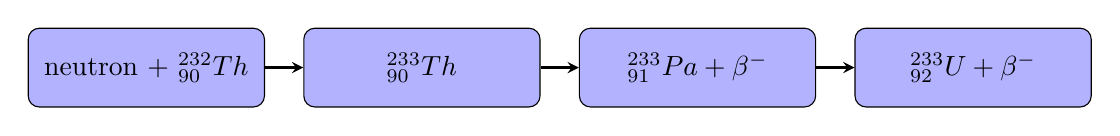
\begin{tikzpicture}[node distance=3.5cm]
\node (th232) [process] {neutron + $^{232}_{90}Th$};
\node (th233) [process, right of=th232] {$^{233}_{90}Th$};
\node (pa233) [process, right of=th233]{$^{233}_{91}Pa + \beta^{-}$};
\node (u233) [process, right of=pa233]{$^{233}_{92}U + \beta^{-}$};

\draw [arrow] (th232) -- (th233); 
\draw [arrow] (th233) -- (pa233);
\draw [arrow] (pa233) -- (u233);

\end{tikzpicture}
\end{figure}


\section{Introduction}


Some of the claims made by papers fail to capture
the entire picture of the fuel cycle, considering they have different
technologies used for each fuel cycle. For example, it is difficult
to compare the `superiority' of a fuel cycle by comparing the 
\gls{LWR} \gls{UNF} of radiotoxicity, since the technologies
representing the fuel cycle is different.

%da fa
The thorium fuel cycle to look at is, namely the EG38
from the Nuclear Fuel Cycle Evaluation and Screening Study \cite{wigeland_nuclear_2014},
which is the continuous recycle of $^{233}U/Th$ with new
Th fuel in both fast and thermal critical reactors.
The reactors that will be used is the \gls{MSBR} \cite{robertson_conceptual_1971},
which includes an online reprocessing facility that
continuously remove \glspl{FP} and \glspl{MA} from the core
and refuels the bred \uthree to maintain criticality. 
The neutrons are moderated by graphite for better breeding.


The uranium-plutonium fuel cycle to be compared is the 
EG23, continuous recycle of U/Pu with new natural uranium
fuel in fast critical reactors. The reactor that will be used
is the \gls{SFR}, with oxide fuel. The \gls{MOX} fuel will 
breed plutonium, which will be recycled into the \gls{SFR}.
The \glspl{FP} and \glspl{MA} will be disposed, and the 
mass loss will be filled with natural uranium.

For a fair comparison, the breeding ratio of the two
reactors should be similar.

\section{Method}

The goal of this study is to calculate sustainability
metrics of the two advanced fuel cycles for comparison.
First, SERPENT simulations of both the \gls{MSBR} and \gls{SFR}
are run with varying parameters. These results are run
through RAVEN \cite{rabiti_mathematical_2013} to generate
a \gls{ROM}, which is then implemented into a \Cyclus
archetype. This \Cyclus archetype then acts as a reactor
module that mimics SERPENT code in executing depletion
calculations as well as output reactor metrics.

Unlike the E\&S Study, this study looks at the 
fuel cycle in a transition scenario, and assesses
the viability and speed of transition as well as
the sustainability metrics of the fuel cycle at equilibrium.

Sustainability metrics are defined as how less of a requirement
from outside sources the fuel cycle needs. Traditional fuel cycle
metrics are: natural resource utilization, natural resource
usage per energy generation, spent fuel and waste radiotoxicity
and volumne.  Additionally, for advanced fuel cycles,
it is necessary to consider all stages of the fuel cycle,
namely reprocessing. Reprocessing takes a large part of the 
cost of advanced fuel cycle. A careful analysis of not only
the economic cost but also the externalities such as the health and societal cost of 
reprocessing should be analyzed for a fuller picture.


\chapter{Literature Review}

Th benefits:
    thermal breeder
    abundance
    non-proliferation
    lower radiotoxicity


Fundamental differences in uranium and thorium fuel
cycles have been discussed in various literature,
their topics ranging from 
non-proliferation
\cite{iaea_thorium_2005} 
\cite{moir_recommendations_2008} 
\cite{kang_u-232_2001} %this guy is skeptical of it
,
availability
\cite{herring_uranium_2013}
,
better neutronic properties (moreso at higher temperatures)
\cite{lung_perspectives_1998}

thermal breeding capability
\cite{robertson_conceptual_1971}
and 
radiotoxicity of spent fuel
\cite{croff_comparative_2016}
.


\subsection{Proliferation Resistance}
Thorium is claimed to have a higher proliferation resistance
due to its diversion barriers. The barriers can be divided into
two categories - intrinsic and extrinsic. Material barriers
are qualities that make it difficult to produce a weapon related
to the composition of the material, along with the difficulty of
access to the material. The IAEA defines a fissile material's weapon
quality by the following three properties: critical mass, spontaneous 
fission yield (weapon degradation), and heat emission \cite{iaea_thoriuim_2005}.
Although \uthree has a lower spontaneous fission rate and decay heat per kilogram,
it has a higher critical mass than that of \pu and is harder to separated.
Thorium breeding leads to a mixture of different uranium isotopes including
\utwo, which is a 2.6 MeV gamma emitter \cite{moir_recommendations_2008}. This hard gamma emitter provides
both a diversion and fabrication barrier, as well as increase the material's detectability
Also, \uthree can be easily diluted by adding abundant natural uranium, while
there is no comparable dilution method for plutonium \cite{kang_u-232_2001}.


\subsection{Availability}
It is estimated that thorium is three to four times more abundant in
nature than uranium \cite{iaea_thorium_2005}.


\cite{herring_uranium_2013}

Other important fuel cycle benefit metrics
such as safety usually attribute heavily
to reactor design, not the fuel. In other words,
it could be said that thorium-fueled \glspl{MSR} are safer
than uranium-fueled \glspl{LWR}, but it is hard to claim
that thorium fuels are inherently `safer' than uranium fuels.

There could be arguments made 

easier to denature \cite{kang_u-232_2001} by adding u238, while
pu is hard to denature because it can't be found in nature



such as safety and 


and reactor design.


The thorium fuel cycle is known to be proliferation
resistant, due to its production of \utwo, which
has daughter products that emit hihg-energy 


Thorium cycle must be initiated.

\chapter{Conclusions}


\appendix*

\include{Appendix.tex}


\bibliographystyle{apalike}
\bibliography{thesisbib}

\end{document}
\endinput
%%
%% End of file `thesis-ex.tex'.
